\subsection{ANFIS Validation} \label{compvis_anfisvalid}

Previous sections (e.g. Section \ref{fusion_bounds}) hypothesised that a physics-informed deep learning fusion network, such as ANFIS, will outperform a standard Naive Bayes (NB) fusion model. It is therefore important to validate this hypothesis with a \textbf{basic} simulation of environmental conditions and the \textit{consequent} sensor data. This simulation aims to demonstrate that an ANFIS network with incorporated domain knowledge can outperform NB, when the sensor data are \textit{not} conditionally independent.

\subsubsection{Synthetic Data Generation}  

    ANFIS is expected to outperform NB because the latter assumes conditional independence between sensors, an assumption often invalid in real-world conditions where there is coupling between the two sensors through the causal physics of the environment. 
    
    To demonstrate NB's limitations, synthetic data is generated to model the influence of \textbf{soil moisture}. As detailed in Section \ref{fuzzy_rules}, increased soil moisture enhances thermal sensor return (via increased thermal conductivity) while inhibiting radar sensor return (via increased electrical conductivity). This is not the only coupling between the two sensors, but modelling one suffices to illustrate the advantages of ANFIS. Additionally, the model includes the effect of wind speed, which decreases thermal returns but does not affect radar returns.


    A 200$\times$200 grid was generated, with 2\% coverage of randomly placed mines. Soil moisture was simulated using a simplified sine-cosine function varying between 0 and 1, and is shown in Figure \ref{fig:anfis_summary}. Wind speed was modelled using random samples from a Gaussian distribution with a mean of 0 and a standard deviation of 2~m/s. Following the layered approach (Section \ref{sec:msp_layered_approach}), the radar sensor only samples points previously flagged by the thermal sensor. To simulate GPS drift and further illustrate the limitations of NB under uncertainty, a small random spatial shift of one cell was introduced between the thermal and radar datasets.


\subsubsection{Sensor Modelling}  

    The sensor confidence maps were computed using equations to model the effects of soil moisture (\textit{m}, dimensionless, ranging 0-1) and wind speed (\textit{w}, in \si{\metre\per\second}) on the thermal and radar sensor outputs. These curves are designed to reflect the higher precision characteristic of the radar sensor and the higher recall of the thermal sensor. Sensor noise was modelled as zero-mean Gaussian white noise ($\mathcal{N}$), with a variance of 0.15 for the thermal sensor, and 0.12 for the radar sensor. The resulting sensor output probabilities are given by:
    
    \begin{equation}
        P_{\text{thermal}} = \begin{cases} 
        0.9 - 0.66e^{-m/40} - 0.02w + \mathcal{N}(0,0.15) & \text{if mine present} \\
        0.6 - 0.48e^{-m/200} - 0.02w + \mathcal{N}(0,0.15) & \text{if no mine}
        \end{cases}
    \end{equation}
    
    \begin{equation}
        P_{\text{radar}} = \begin{cases}
        1.2 \cdot 0.6e^{-m/60} + \mathcal{N}(0,0.12) & \text{if mine present} \\
        0.45 \cdot 0.6e^{-m/60} + \mathcal{N}(0,0.12) & \text{if no mine}
        \end{cases}
    \end{equation}

\subsubsection{Fusion Implementation}

    \paragraph{ANFIS} The ANFIS architecture is implemented using the Keras framework \footnote{\url{https://keras.io/}}. The model accepts four input features: soil moisture, wind speed, thermal sensor confidence, and radar sensor confidence. Input fuzzification uses three Gaussian membership functions per input, whose parameters ($c,~\sigma$ in Equation \ref{eq:gaussian_mf}) are trainable variables within the network.

    While Section \ref{ANFIS} proposed explicit, physics-derived fuzzy rules, this basic implementation uses a dense rule antecedent layer (see Figure \ref{fig:ANFIS_diagram}). A dense layer combines the membership degrees from the four inputs (each with 3 membership functions), allowing the network to learn the antecedent combinations corresponding to all $3^4=81$ possible fuzzy rules. The consequent layer learns the parameters that define the output for each of these implicitly formed rules. 
    
    The final custom output layer calculates a normalised, weighted sum of these rule outputs and applies a sigmoid function to ensure the final fused confidence is between 0 and 1.

    \paragraph{NB} The Naive Bayes (NB) fusion method combines the thermal and radar sensor confidence values $P_{\text{thermal}}$, $P_{\text{radar}}$. Assuming conditional independence between the sensors given the presence or absence of a mine, the fused confidence $P_{\text{fused}}$ is calculated using Bayes Theorem, which may be written as:

    \begin{equation}
        \label{eq:bayes_fusion}
        \mathcal{P}_\text{fused} = \frac{\mathcal{P}_\text{thermal}\mathcal{P}_\text{radar}}{\mathcal{P}_\text{thermal}\mathcal{P}_\text{radar} + (1-\mathcal{P}_\text{thermal})(1-\mathcal{P}_\text{radar})}
    \end{equation}
    
\subsubsection{Results and Conclusion}  

    The ANFIS model demonstrated improved recall (ANFIS: 0.66 NB: 0.11) and precision (ANFIS: 0.92 NB: 0.28), compared to Naive Bayes. The surprisingly low NB performance is partly caused by the random shifting between the radar the thermal maps, that means NB often gives null results from multiplying misaligned confidence values. However, more fundamentally, the simulation highlights ANFIS' key advantage; it can leverage the environmental context (soil moisture and wind speed inputs in this implementation) to implicitly model the physical coupling between sensor readings. Naive Bayes' inability to handle uncertainty and conditionally dependent data is also clear. See the predicted mine locations from each fusion algorithm in Figure \ref{fig:anfis_summary}.

     While this simulation is simplified, it validates the hypothesis that a deep learning fusion architecture, constrained to physically-plausible solutions and incorporates environmental context \textbf{can perform significantly better than purely statistical methods}, like Naive Bayes.

    \begin{figure}[h]
        \centering
        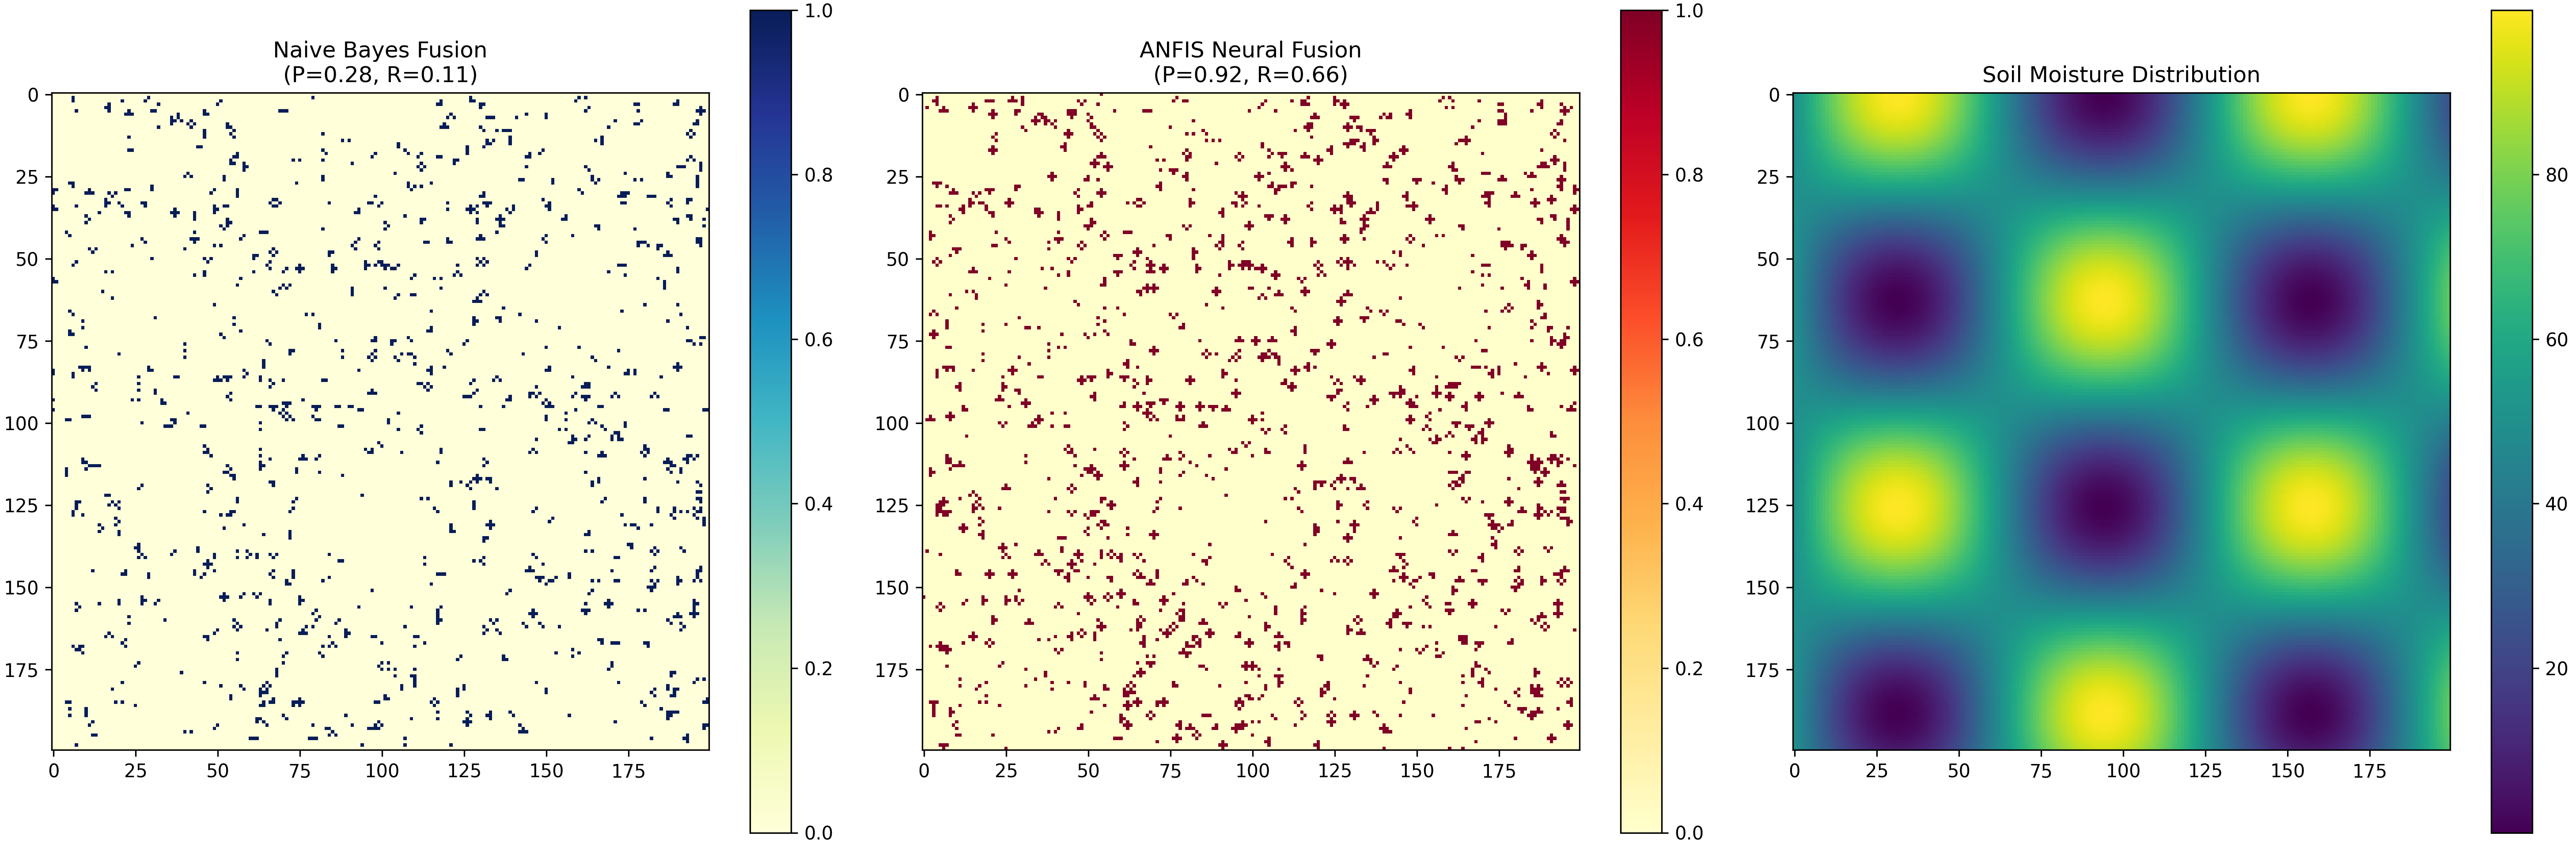
\includegraphics[width=0.98\textwidth]{figs/Rory/0_summary.png}
        \caption[ANFIS NB comparison summary]{ANFIS NB comparison summary. \textbf{Left:} simulated fusion for Naive Bayes. \textbf{Centre:} simulated fusion for ANFIS. \textbf{Right:} soil moisture distribution}
        \label{fig:anfis_summary}
    \end{figure}

    \paragraph{Future Work} 

        Several other physics-driven fusion algorithms exist. Another such approach is Physics Based Deep Learning (PBDL)\footnote{\url{https://www.physicsbaseddeeplearning.org/intro.html}}, which benefits from implementing the physical domain knowledge at a deeper level in the \textit{model architecture and loss function}. PBDL is a recent field in Artificial Intelligence (AI), and it may have significant benefits, such as greater robustness to environmental variations in data-fusion for the detection of landmines.
